\documentclass[10pt,a4paper]{article}
\usepackage{amsmath}
\usepackage{amssymb}
\usepackage{graphicx}
\usepackage{color}
\usepackage{fancyhdr}
\usepackage{fancyvrb}
\usepackage[margin=3.5cm]{geometry}
\usepackage{framed}
\usepackage{enumerate}
\usepackage{textcomp}
\def\ket#1{\left|#1\right\rangle}
\def\bra#1{\left\langle#1\right|}
\def\braket#1{\left\langle#1\right\rangle}

\definecolor{linkcol}{rgb}{0.0, 0.0, 0.7}
\usepackage[colorlinks=true,urlcolor=linkcol,citecolor=black,linkcolor=linkcol]{hyperref}

\setcounter{section}{4}
\renewcommand\thesection{\arabic{section}}
\renewcommand\thesubsection{\thesection.\arabic{subsection}}

\fancyhf{}
\lhead{\tiny Y.~D.~Chong (2020)}
\rhead{\scriptsize MH2801: Complex Methods for the Sciences}
\lfoot{}
\rfoot{\thepage}
\pagestyle{fancy}

\begin{document}
\setcounter{page}{38}

\section{Complex Waves}
\label{complex-waves}

Just as complex numbers provide a convenient way to study
oscillations, they can also be employed to model wave motion. In
physics, complex numbers are commonly used in the study of
electromagnetic (light) waves, sound waves, and other kinds of waves.


\subsection{The wave equation}
\label{the-wave-equation}

A wave can be described by a function $f(x,t)$, called a
\textbf{wavefunction}, which specifies the value of a measurable
physical quantity at each position $x$ and time $t$. For simplicity,
we will assume that space is one-dimensional, so $x$ is a single real
number. We will also assume that $f(x,t)$ is a number, rather than a
more complicated object such as a vector. For instance, a sound wave
can be described by a wavefunction $f(x,t)$ representing the air
pressure at each point of space and time.

The evolution of the wavefunction is described by a partial
differential equation (PDE) called the \textbf{time-dependent wave
  equation}:
\begin{equation}
\frac{\partial^2 f}{\partial x^2} = \frac{1}{v^2} \frac{\partial^2 f}{\partial t^2}, \;\;\; v \in\mathbb{R}^+.
\end{equation}
The parameter $v$, which we take to be a positive real constant, is
called the \textbf{wave speed}, for reasons that will shortly become
clear.

Sometimes, we re-arrange the wave equation into the following form,
consisting of a linear differential operator acting on $f(x,t)$:
\begin{equation}
\left(\frac{\partial^2}{\partial x^2} - \frac{1}{v^2} \frac{\partial^2}{\partial t^2}\right) \; f(x,t) = 0.
\end{equation}
This way of writing the wave equation emphasizes that it is a linear
PDE, meaning that any linear superposition of solutions is likewise a
solution.

\subsection{Real solutions to the wave equation}
\label{real-solutions-to-the-wave-equation}

We first consider real solutions to the wave equation. One family of
solutions are \textbf{travelling waves} of the form
\begin{equation}
f(x,t) = f_0 \, \cos\!\big(kx - \omega t + \phi\big),\quad\mathrm{where}\;\, \left|\frac{\omega}{k}\right| = v.
\label{realsol}
\end{equation}
By direct substitution, we can verify that this satisfies the PDE. We
call $f_0$ the \textbf{amplitude} of the wave, $\phi$ the
\textbf{phase}, $\omega$ the (angular) \textbf{frequency}, and $k$
the \textbf{wavenumber}. By convention, $\omega$ is taken to be a
positive real number. However, $k$ can be either positive or
negative, and its sign determines the direction of propagation of the
wave; the magnitude of the wavenumber is inversely related to the
wavelength $\lambda$ by $\lambda = 2\pi/|k|$.
    
As $t$ increases, the wave moves to the right if $k$ is positive,
whereas it moves to the left if $k$ is negative. Here's one way to
reason out why this is the case. Consider introducing a small change
in time, $\delta t$, into the function $\cos(kx - \omega t +
\phi)$. If, together with this time shift, we change $x$ by $\delta x
= (\omega/k)\, \delta t$, then the change in the $kx$ term and the
change in the $\omega t$ term cancel, leaving the value of the cosine
unchanged:

\begin{figure}[ht]
  \centering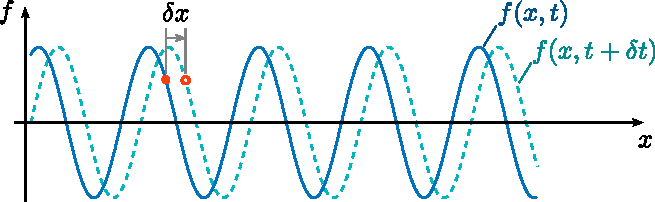
\includegraphics[width=0.6\textwidth]{wave_velocity}
\end{figure}

\noindent
This implies that the wave shifts by $\delta x = (\omega/k)\, \delta
t$ during the time interval $\delta t$. Hence, the wave velocity is
\begin{equation}
\textrm{velocity} = \frac{\delta x}{\delta t} = \frac{(\omega/k)\,\delta t}{\delta t} = \frac{\omega}{k}.
\end{equation}
As previously noted, $\omega$ is conventionally taken to be a positive
real number. Hence, positive $k$ implies that the wave is right-moving
(positive velocity), and negative $k$ implies the wave is left-moving
(negative velocity). Moreover, the wave speed is the absolute value of
the velocity, which is precisely equal to the constant $v$:
\begin{equation}
\textrm{speed}\; = \, \left|\frac{\delta x}{\delta t}\right| = \frac{\omega}{\left|k\right|} = v.
\end{equation}

\subsubsection{Standing waves}
\label{standing-waves}

Suppose we have two travelling wave solutions, with equal amplitude and
frequency, moving in opposite directions:
\begin{equation}
f(x,t) = f_0 \, \cos(kx - \omega t + \phi_1) + f_0 \cos(-kx - \omega t + \phi_2).
\end{equation}
Here, we denote $k = \omega/c$. Such a superposition is also a
solution to the wave equation, called a \textbf{standing wave}. It can
be re-written in a variable-separated form (i.e., as the product of a
function of $x$ and a function of $t$):
\begin{equation}
f(x,t) = 2f_0 \, \cos\big[kx + (\phi_1-\phi_2)/2\big]\, \cos\big[\omega t - (\phi_1+\phi_2)/2\big].
\label{standingsol}
\end{equation}
This can be proven using the trigonometric addition formulas, but the
proof is tedious.

\subsection{Complex solutions to the wave equation}
\label{complex-solutions-to-the-wave-equation}

It is much easier to deal with the wave equation if we promote it into a
complex PDE by letting $f(x,t)$ take on complex values. However, $x$
and $t$ will remain real. We will also take the wave speed $v$ to be
real, for now.

From any complex solution to the wave equation, we can take the real
part to get a solution to the real PDE, thanks to linearity (see
Section 3.1):
\begin{equation}
\left(\frac{\partial^2}{\partial x^2} - \frac{1}{v^2} \frac{\partial^2}{\partial t^2}\right) \mathrm{Re}\left[f(x,t)\right] = \mathrm{Re} \left[ \left(\frac{\partial^2}{\partial x^2} - \frac{1}{v^2} \frac{\partial^2}{\partial t^2}\right) f(x,t)\right] = 0.
\end{equation}
There exists a nice set of complex solutions to the wave equation,
called \textbf{complex travelling waves}, which take the form
\begin{equation}
f(x,t) = A \, e^{i(kx - \omega t)} \quad\mathrm{where}\;\; \left|\frac{\omega}{k}\right| = v.
\end{equation}
It can be verified by direct substitution that this satisfies the PDE.
The complex constant $A$ is called the \textbf{complex amplitude} of
the wave. Consider what happens if we take the real part of the above
solution:
\begin{equation}
\begin{aligned}\mathrm{Re}\Big\{A \, e^{i(kx - \omega t)}\Big\} &= \mathrm{Re}\Big\{ |A|\, e^{i\mathrm{arg}[A]} \; e^{i(kx - \omega t)}\Big\} \\ &= \big|A\big|\; \mathrm{Re}\Big\{ e^{i\mathrm{arg}[A]} \, e^{i(kx - \omega t)}\Big\} \\ &= \big|A\big|\; \cos\big(kx - \omega t + \mathrm{arg}[A]\big)\end{aligned}
\end{equation}
Comparing this to Eq.~\eqref{realsol}, we see that $|A|$ serves as the
amplitude of the real wave, while $\mathrm{arg}(A)$ serves as the
phase factor $\phi$. Mathematically, the complex solution is more
succinct than the real solution: a single complex parameter $A$
combines the roles of two parameters in the real solution.

The complex representation also makes wave superpositions easier to
handle. As an example, consider the superposition of two
counter-propagating waves of equal amplitude and frequency, with
arbitrary phases. Using complex travelling waves, we can calculate the
superposition with a few lines of algebra:
\begin{equation}
\begin{aligned}f(x,t) &= \displaystyle \big|A\big| \, e^{i(kx - \omega t + \phi_1)} + \big|A\big| \, e^{i(-kx - \omega t + \phi_2)} \\ &= \displaystyle \big|A\big|\, \left(e^{i(kx + \phi_1)} + e^{-i(kx - \phi_2)}\right)\, e^{-i\omega t} \\ &= \displaystyle \big|A\big|\, \left(e^{i[kx + (\phi_1-\phi_2)/2]} + e^{-i[kx + (\phi_1 - \phi_2)/2]}\right)\, e^{i(\phi_1 + \phi_2)/2} \,e^{-i\omega t} \\ &= \displaystyle 2\big|A\big|\, \cos\left[kx + (\phi_1-\phi_2)/2\right] \,e^{-i[\omega t -(\phi_1+\phi_2)/2]}\end{aligned}
\end{equation}
Taking the real part yields Eq.~\eqref{standingsol}, without the need
for tedious manipulations of trigonometric formulas.

\subsection{Waves in 3D space}
\label{waves-in-3d-space}

The wave equation can be generalized to three spatial dimensions by
replacing $f(x,t)$ with a wavefunction that depends on three spatial
coordinates, $f(x,y,z,t)$. The second-order derivative in $x$ is then
replaced by second-order derivatives in each spatial direction:
\begin{equation}
\left(\frac{\partial^2}{\partial x^2} + \frac{\partial^2}{\partial y^2} + \frac{\partial^2}{\partial z^2} - \frac{1}{v^2} \frac{\partial^2}{\partial t^2}\right) \; f(x,y,z,t) = 0.
\label{3dwave}
\end{equation}
This PDE supports complex plane wave solutions of the form
\begin{equation}
f(x,y,z,t) = A \, e^{i(\vec{k} \cdot \vec{r} - \omega t)},
\end{equation}
where
\begin{equation}
\vec{k} = \begin{bmatrix}k_x\\k_y\\k_z\end{bmatrix}, \;\;\; \vec{r} = \begin{bmatrix}x\\y\\z\end{bmatrix}, \;\;\;\frac{\omega}{\sqrt{k_x^2 + k_y^2 + k_z^2}} = v.
\end{equation}
Again, we can verify that this is a solution by direct
substitution. We call $\vec{k}$ the \textbf{wave-vector}, which
generalizes the wavenumber $k$. The direction of the wave-vector
specifies the spatial direction in which the wave travels.

\subsection{Harmonic waves}
\label{harmonic-waves}

We are often interested in waves undergoing \textbf{harmonic
oscillation}, i.e.~varying sinusoidally with a constant frequency
$\omega$ everywhere in space. Such waves can be described by
wavefunctions of the form
\begin{equation}
f(x,y,z,t) = \psi(x,y,z) \, e^{-i\omega t}.
\end{equation}
By writing the wavefunction in this form, we are performing a separation
of variables between $\vec{r}$ and $t$. This is a common method for
simplifying PDEs, and is justified by the linearity of the wave
equation. If we can find harmonic solutions for each frequency
$\omega$, we can linearly combine them to construct more general
solutions that are non-harmonic.

By direct substitution into Eq.~\eqref{3dwave}, we can show that
$\psi(x)$ obeys
\begin{equation}
\left[\frac{\partial^2}{\partial x^2} + \frac{\partial^2}{\partial y^2} + \frac{\partial^2}{\partial z^2} + \left(\frac{\omega}{v}\right)^2\right] \, \psi(x,y,z) = 0.
\end{equation}
This is related to the original time-dependent wave equation by the
replacement of $\partial/\partial t$ with $-i\omega$.

\subsubsection{Waves in complex media}
\label{waves-in-complex-media}

So far, our discussion has been limited to waves propagating in a
uniform, energy-conserving medium with a fixed wave speed $v$.  There
are two important generalizations of this scenario: (i) non-uniform
media, in which the wave speed varies with position, and (ii) energy
non-conserving media, in which the waves lose or gain energy as they
propagate. To capture these phenomena, we replace the constant $v$ by
\begin{equation}
v = \frac{c}{n},
\end{equation}
where $n$ is called the \textbf{refractive index}, and the constant
$c$ is the wave speed in the limit $n = 1$. In the case of
electromagnetic waves, $c$ is the speed of light in a vacuum.

If the refractive index is now allowed to vary with position, the wave
equation in the harmonic representation becomes
\begin{equation}
\left[\frac{\partial^2}{\partial x^2} + \frac{\partial^2}{\partial y^2} + \frac{\partial^2}{\partial z^2} + n^2(x,y,z)\, \left(\frac{\omega}{c}\right)^2\right] \, \psi(x,y,z) = 0.
\end{equation}

\subsubsection{Wave amplification and attenuation}
\label{gainloss}

By allowing the refractive index $n$ to be \emph{complex}, the wave
equation can describe the phenomena of \textbf{wave amplification}
(which is also called \textbf{gain}) and \textbf{wave attenuation} (also
called \textbf{loss}). Amplified and attenuated waves occur in many
different contexts in physics; for example, the amplification of light
waves is the underlying basis for the laser.

To study these phenomena, let us go back to one-dimensional space and
the simple scenario of a position-independent refractive index. For
harmonic waves, the wave equation reduces to
\begin{equation}
\left[\frac{d^2}{d x^2} + n^2\, \left(\frac{\omega}{c}\right)^2\right] \, \psi(x) = 0.
\end{equation}
We now let $n$ be complex, while keeping $\omega$ and $c$ as
positive real numbers. The solutions to the ODE have the form
\begin{equation}
\psi(x) = A \exp\left(\pm \frac{in\omega}{c}x\right),\;\;\;\mathrm{where}\;\; A \in \mathbb{C}.
\label{eq:gainloss-wave}
\end{equation}
Let us write the complex refractive index as
\begin{equation}
n = n' + i n'',\quad \textrm{where}\;\, n',n'' \in \mathbb{R}.
\end{equation}
Then
\begin{equation}
\psi(x) = A \exp\left[\pm in'(\omega/c)x\right]\, \exp\left[\mp n''(\omega/c)x\right].
\end{equation}
The first exponential factor describes the oscillation of the
wavefunction, with the $\pm$ sign determining whether the harmonic
wave is moving to the right or to the left. The second exponential
describes the amplification or attenuation of the wave. If
$n'' \ne 0$, the amplitude varies exponentially with $x$. Thus,
depending on the signs of the various parameters, the wave might grow
exponentially along its direction of propagation, which corresponds to
amplification, or decrease exponentially along its direction of
propagation, which corresponds to damping.

\subsection{Exercises}
\label{exercises}

\begin{enumerate}
\item
  Consider the 1D wave equation in a enclosed box of length $L$ and
  uniform refractive index $n\in\mathbb{R}$. The walls of the box are
  at $x = -L/2$ and $x = L/2$, and the wavefunction goes to zero at
  these points: $\psi(\pm L/2) = 0$ (i.e., Dirichlet boundary
  conditions). Show that $\psi(x) = 0$ for all $x$, \emph{except}
  for certain discrete values of the frequency $\omega$. Find these
  frequencies, and the corresponding non-zero solutions $\psi(x)$.

\item
  As discussed in Section~\ref{gainloss}, a harmonic travelling wave
  in an energy-nonconserving medium is described by
  \begin{equation}
    \left[\frac{d^2}{d x^2} + n^2\, \left(\frac{\omega}{c}\right)^2\right] \, \psi(x) = 0,
  \end{equation}
  where $n$ is a complex number. (As usual, $\omega$ and $c$ are
  assumed to be positive real numbers.) Show that the relative sign of
  $\mathrm{Re}(n)$ and $\mathrm{Im}(n)$ determines whether the wave
  experiences amplification or dissipation, and that the result does
  not depend of the wave's propagation direction.
  \hfill{\scriptsize [solution~available]}

\item
  When the refractive index is complex, can the real part of the
  complex wavefunction be regarded as the solution to the same wave
  equation? If not, derive a real differential equation whose solution
  is the real part of Eq.~\eqref{eq:gainloss-wave}.
\end{enumerate}

    
\end{document}
